
%%%%%%%%%%%%%%%%%%%%%%%%%%%%%%%%%%%%%%%%%
% Beamer Presentation
% LaTeX Template
% Version 1.0 (10/11/12)
%
% This template has been downloaded from:
% http://www.LaTeXTemplates.com
%
% License:
% CC BY-NC-SA 3.0 (http://creativecommons.org/licenses/by-nc-sa/3.0/)
%
%%%%%%%%%%%%%%%%%%%%%%%%%%%%%%%%%%%%%%%%%

%----------------------------------------------------------------------------------------
%	PACKAGES AND THEMES
%----------------------------------------------------------------------------------------

\documentclass[xcolor=table]{beamer}

\usepackage{tikz}
\setbeamertemplate{background canvas}{\begin{tikzpicture}\node[opacity=.3]{
\includegraphics
		[width=\paperwidth]{imagenes/background2.png}};\end{tikzpicture}}

%\setbeamertemplate{background}
%{
\includegraphics[width=\paperwidth,height=\paperheight,keepaspectratio]{imagenes/background2.png}}

\mode<presentation> {
	
	% The Beamer class comes with a number of default slide themes
	% which change the colors and layouts of slides. Below this is a list
	% of all the themes, uncomment each in turn to see what they look like.
	
	%\usetheme{default}
	%\usetheme{AnnArbor}
	%\usetheme{Antibes}
	%\usetheme{Bergen}
	%\usetheme{Berkeley}
	%\usetheme{Berlin}
	%\usetheme{Boadilla}
	%\usetheme{CambridgeUS}
	%\usetheme{Copenhagen}
	%\usetheme{Darmstadt}
	%\usetheme{Dresden}
	%\usetheme{Frankfurt}
	%\usetheme{Goettingen}
	%\usetheme{Hannover}
	%\usetheme{Ilmenau}
	%\usetheme{JuanLesPins}
	%\usetheme{Luebeck}
	\usetheme{Madrid}
	%\usetheme{Malmoe}
	%\usetheme{Marburg}
	%\usetheme{Montpellier}
	%\usetheme{PaloAlto}
	%\usetheme{Pittsburgh}
	%\usetheme{Rochester}
	%\usetheme{Singapore}
	%\usetheme{Szeged}
	%\usetheme{Warsaw}
	
	% As well as themes, the Beamer class has a number of color themes
	% for any slide theme. Uncomment each of these in turn to see how it
	% changes the colors of your current slide theme.
	
	%\usecolortheme{albatross}
	%\usecolortheme{beaver}
	%\usecolortheme{beetle}
	%\usecolortheme{crane}
	%\usecolortheme{dolphin}
	%\usecolortheme{dove}
	%\usecolortheme{fly}
	%\usecolortheme{lily}
	%\usecolortheme{orchid}
	%\usecolortheme{rose}
	%\usecolortheme{seagull}
	%\usecolortheme{seahorse}
	%\usecolortheme{whale}
	%\usecolortheme{wolverine}
	
	%\setbeamertemplate{footline} % To remove the footer line in all slides uncomment this line
	%\setbeamertemplate{footline}[page number] % To replace the footer line in all slides with a simple slide count uncomment this line
	
	%\setbeamertemplate{navigation symbols}{} % To remove the navigation symbols from the bottom of all slides uncomment this line
}

\usepackage{graphicx} % Allows including images
\usepackage[spanish]{babel}
\usepackage{booktabs} % Allows the use of \toprule, \midrule and \bottomrule in tables
\usepackage{multirow}

\usepackage{mathabx}

\usepackage{listings}
\usepackage{float}
\usepackage{amsfonts}

\usepackage{subfigure}
\usepackage{enumerate}
\usepackage{pdfpages}
\usepackage{verbatim} 
\usepackage{enumerate}

%\SetKwFor{For}{para}{hacer}{fin}





%----------------------------------------------------------------------------------------
%	TITLE PAGE
%----------------------------------------------------------------------------------------

\title[]{Metodolog\'ia para estimar p\'erdida de
	carbono a trav\'es de procesamiento de im\'agenes
	satelitales. Caso de uso Chaco Paraguayo} % The short title appears at the bottom of every slide, the full title is only on the title page

\author{Santiago Vera Aquino} % Your name
\institute[FP-UNA] % Your institution as it will appear on the bottom of every slide, may be shorthand to save space
{
	Universidad Nacional de Asunci\'on \\ % Your institution for the title page
	Facultad Polit\'ecnica \\
	Ingenier\'ia en Inform\'atica \\
	\medskip
	\textit{Proyecto Final de grado} % Your email address
}
\date{\today} % Date, can be changed to a custom date

\begin{document}
	
	\begin{frame}
		\titlepage % Print the title page as the first slide
	\end{frame}
	
	%------------------------------------------------
	
	\begin{frame}
		\frametitle{Contenido}
		\tableofcontents % Write out the Table of Contents	
	\end{frame}
	
	\section{Conceptos generales}
	%------------------------------------------------
	\begin{frame}
		\frametitle{Conceptos generales\\Cambio Clim\'atico}
		
		\begin{figure}
			\centering
			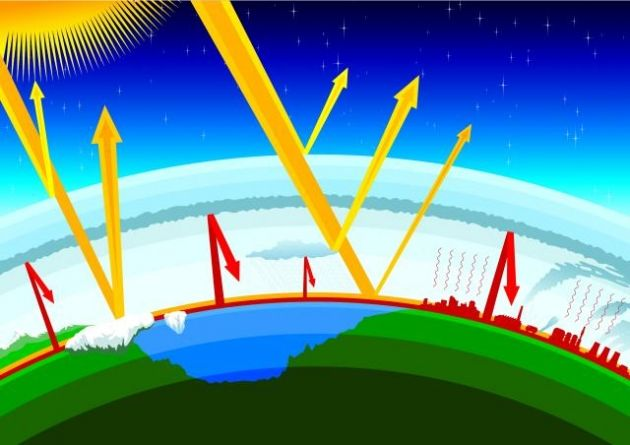
\includegraphics[width=0.7\linewidth]{imagenes/cap2/calentamientoGlobal}
			\label{fig:calentamientoGlobal}
		\end{figure}
	\end{frame}
	
	%%%%%%%%%%%%%
	
	\begin{frame}
		\frametitle{Conceptos generales\\Ciclo de carbono}		
		\begin{figure}
			\centering
			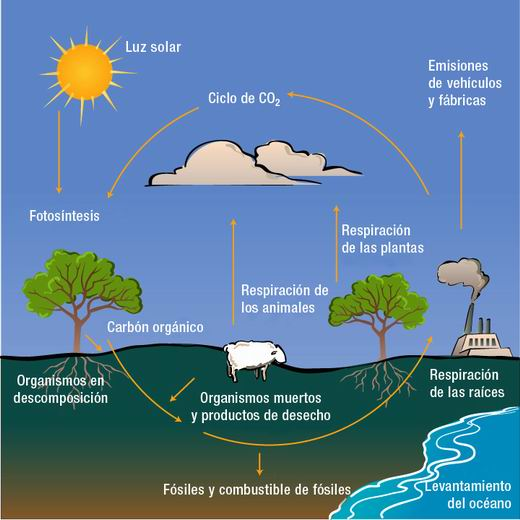
\includegraphics[width=0.5\linewidth]{imagenes/cicloCarbono}
			\label{fig:cicloCarbono}
		\end{figure}
	\end{frame}
	
	
	%%%%%%%%%%%%%
	
	\begin{frame}
		\frametitle{Conceptos generales\\Medici\'on de balances de carbono}		
		\begin{itemize}
			\item \textbf{Inventarios forestales.} 
			\begin{figure}[h!]
				\centering
				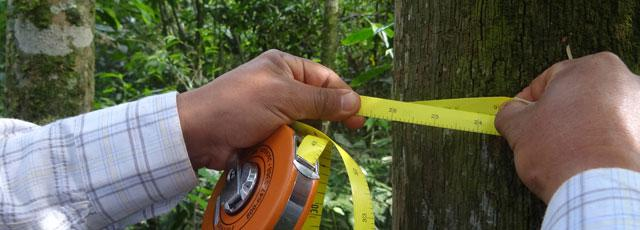
\includegraphics[width=0.7\linewidth]{imagenes/inventario-forestal}
				\label{fig:inventario-forestal}
			\end{figure}
			
			\item \textbf{Sensores remotos.} 
			\begin{figure}[h!]
				\centering
				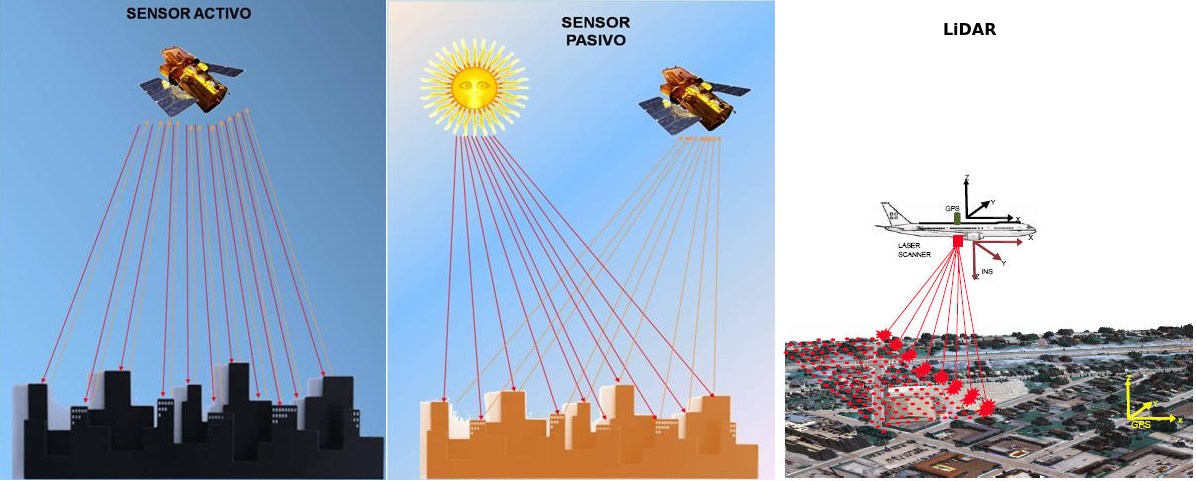
\includegraphics[width=0.7\linewidth]{imagenes/sensores}
				
				\label{fig:sensores}
			\end{figure}
			
		\end{itemize}
	\end{frame}
	
	%%%%%%%%%%%%%
	
	\begin{frame}
		\frametitle{Conceptos generales\\Teledetecci\'on en el medio ambiente}		
		\begin{figure}[H]
			\centering
			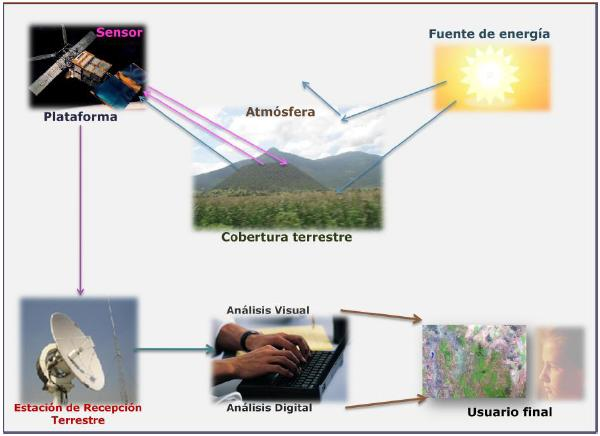
\includegraphics[width=0.7	\textwidth]{imagenes/cap3/teledeteccion.png}
			\label{fig:tele}
		\end{figure}
	\end{frame}
	
	%%%%%%%%%%%%%
	\section{Motivaci\'on}
	\begin{frame}
		\frametitle{Motivaci\'on}		
		Actividades principales del REDD+:
		\begin{itemize}
			\item Evitar p\'erdidas como emisiones de gases de efecto invernadero (conservaci\'on, no deforestaci\'on, no degradaci\'on).
			\item Mantener el dep\'osito o stock de carbono (conservaci\'on, gesti\'on sostenible).
			\item Incrementar el dep\'osito por su efecto de retenci\'on o sumidero de carbono (conservaci\'on, restauraci\'on, gesti\'on sostenible).
		\end{itemize}
		
	\end{frame}
	
	%%%%%%%%%%%%%
	\section{Trabajos relacionados}
	\begin{frame}
		\frametitle{Trabajos relacionados}		
		
		\begin{table}
			\scalebox{0.35}{
				\begin{tabular}{|p{8cm}|p{8cm}|p{8cm}|p{8cm}|p{8cm}|}
					
					\hline
					\textbf{A\~{n}o}& \textbf{Autores} & \textbf{Trabajo} & \textbf{Evaluaciones} \\
					\hline \hline
					2009          & Huang et al.                                           & Assessment of Paraguay's forest cover change using Landsat observations                                                                                                & Presiciones globales mayores al $90\%$ y errores por comisi\'on menores al $10\%$         \\ \hline
					2010          & Matthew L. Clark et al.                                & A scalable approach to mapping annual land cover at 250 m using MODIS time series data: A case study in the Dry Chaco ecoregion of South America                       & Presici\'on global del $79\%$                                                             \\ \hline
					2011          & Saatchi et al.                                         & Benchmark map of forest carbon stocks in tropical regions across three continents                                                                                      & Incertidumbre media en las estimaciones del 30\%                                          \\ \hline
					2012          & Gustavo Miguel Huespe Duarte                           & Detecci\'on de cambios de la cobertura vegetal mediante \'indices de vegetaci\'on (NDVI), dentro y fuera de la Reserva de la biosfera del Chaco en el periodo 1985-2011  & Presenta conclusiones acerca del cambio detectado en diferentes regiones del caso de estudio.                                                                               \\ \hline
					2012          & Nancy L. Harris et al.                                 & Baseline map of carbon emissions from deforestation in tropical regions                                                                                                & Intervalo de predicci\'on entre $ 0.57 $ a $ 1.22 $ (Pg C year$ ^{-1} $)                      \\ \hline
					2013          & ParLu, WWF Paraguay y la Facultad de Ciencias Agrarias & Desarrollo del estudio de linea de base para el sitio 	piloto Bosque atl\'antico de Alto Paran\'a. (BAAPA)                                                               & Coeficiente de determinaci\'on entre el NDVI y carbono r2=0.64                              \\ \hline
					
					2013          & Clovis Grinand et al.                                  & Estimating deforestation in tropical humid and dry forests in Madagascar from 2000 to 2010 using multi-date Landsat satellite images and the random forests classifier & Error de comisi\'on del 85\% para coberturas estables y 61\% para coberturas con cambios. \\ \hline
					2013          & Dolors Armenteras et al.                               & National and regional determinants of tropical deforestation in Colombia                                                                                               & Coeficientes de determinaci\'ons por regiones del pa\'is.                                 \\ \hline
					2014          & Xiao-Peng Song et al.                                  & Annual detection of forest cover loss using time series satellite measurements of percent tree cover                                                                   & Coeficientes de determinaci\'on entre $ 0.7 - 0.9 $                                       \\ \hline
					2014           & Vanessa Almando Dur\'e                                 & Estimaci\'on de carbono almacenado en el Parque Nacional Defensores del Chaco seg\'un formaci\'on vegetal mediante im\'agenes satelitales, a\~{n}o 2014              & Coeficientes de determinac\'on $ r_{1}^{2}=0.8$, $ r_{2}^{2}=0.7 $, $r_{3}^{2}=0.8 $      \\ \hline
					
					2015          & Tyukavina et al.                                       & Aboveground carbon loss in natural and managed tropical 	forests from 2000 to 2012                                                                                      & Incertidumbre en los valores estimados de $ \pm 8 $\%                                     \\ \hline
					2015          & R\'ejou-M\'echain et al.                       & Using repeated small-footprint LiDAR acquisitions to infer spatial and temporal variations of a high-biomass Neotropical forest                                        & RMS 14\% y 23\% en las pruebas.                                                          \\ \hline
					2015          & Jean Pierre Ometto et al.                              & Amazon forest biomass density maps: tackling the uncertainty in carbon emission estimates                                                                              & Incertidumbre en los valores estimados de $ \pm 15\% $ y $ \pm 14\% $                     \\ \hline
					2015          & Michael W. Palace et al.                               & Estimating forest structure in a tropical forest using field measurements, a synthetic model and discrete return lidar data                                            & Coeficientes de determinaci\'on $ r^{2}=0,17 $, $ r^{2}=0,51 $, $ r^{2}=0,43 $            \\ \hline
					2015          & Gu et al.                                         & Downscaling 250-m MODIS Growing Season NDVI Based on Multiple-Date Landsat Images and Data Mining Approaches                                                           & Coeficiente de determinaci\'on $ r^{2}=0.97 $                                             \\ \hline		 
				\end{tabular}}
				
			\end{table}
			
			
		\end{frame}
		
		%%%%%%%%%%%%%
		\section{Objetivos}
		\begin{frame}
			\frametitle{Objetivos}		
			\begin{itemize}
				\item \textbf{Objetivos generales}
				\begin{itemize}
					\item Desarrollar una metodolog\'ia autom\'atica de an\'alisis de im\'agenes satelitales multitemporales para la generaci\'on de indicadores respecto a la p\'erdida del contenido de carbono en zonas del Chaco Paraguayo.
					\item Dise\~{n}ar un m\'etodo de detecci\'on de cambio forestal automatizada entre secuencias multitemporales de im\'agenes satelitales. 
				\end{itemize}
				\item \textbf{Objetivos espec\'ificos}
				\begin{itemize}
					\item Establecer normalizaciones de im\'agenes para la comparaci\'on multitemporal. 
					\item Determinar una constante para la clasificaci\'on de vegetaci\'on en im\'agenes satelitales.
					\item Determinar la relaci\'on entre el NDVI y el carbono a trav\'es de muestreos.
					\item Evaluar la detecci\'on de cambio forestal con el estado del arte. 	
				\end{itemize}
				
			\end{itemize}
			
		\end{frame}
		
		%%%%%%%%%%%%%
		\section{Im\'agenes satelitales}
		\begin{frame}
			\frametitle{Im\'agenes satelitales\\Sensores remotos}
			\begin{itemize}
				\item \textbf{Resoluci\'on espacial} 
				\begin{figure}[H]
					\centering
					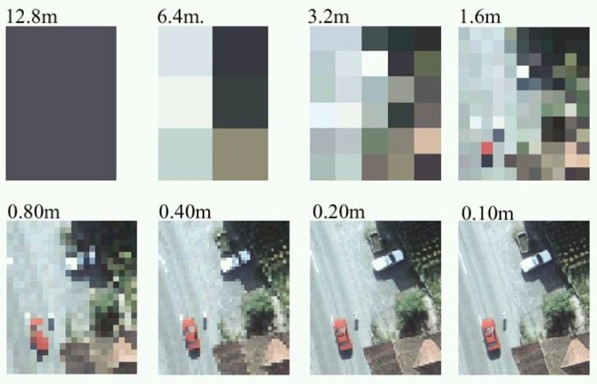
\includegraphics[width=0.4	\textwidth]{imagenes/cap3/resolucion_espacial_n.jpg}
					\label{fig:espatialRes}
				\end{figure}
				\item \textbf{Resoluci\'on espectral} 
				\begin{figure}[H]
					\centering
					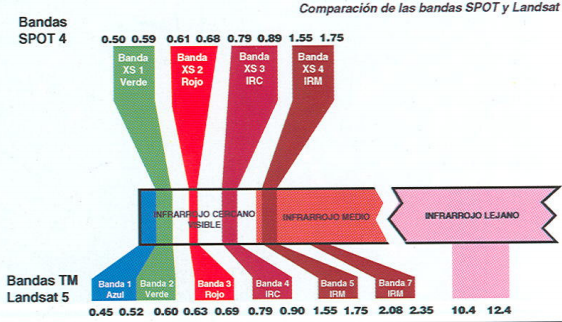
\includegraphics[width=0.4	\textwidth]{imagenes/cap3/espectral_spot_landsat.png}
					\label{fig:espectralRes}
				\end{figure}
			\end{itemize}		
			
		\end{frame}
		
		\begin{frame}
			\frametitle{Im\'agenes satelitales\\Sensores remotos}
			\begin{itemize}
				
				\item \textbf{Resoluci\'on radiom\'etrica}
				\begin{figure}[H]
					\centering
					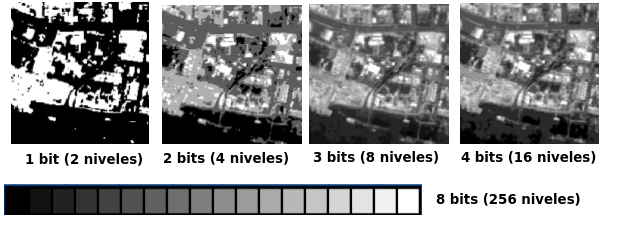
\includegraphics[width=0.5	\textwidth]{imagenes/cap3/radiometrica_bits}
					\label{fig:radioRes}
				\end{figure}
				\item \textbf{Resoluci\'on temporal} 
				\begin{figure}[H]
					\centering
					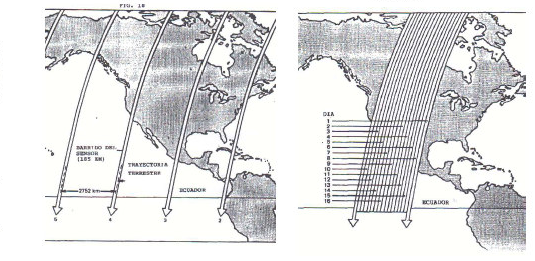
\includegraphics[width=0.5	\textwidth]{imagenes/cap3/resolucion_temporal_land.png}
					\label{fig:temporaRes}
				\end{figure}
			\end{itemize}		
			
		\end{frame}
		
		%%%%%%%%%%%%%
		\begin{frame}
			\frametitle{Im\'agenes satelitales\\Definici\'on}		
			Una imagen satelital es una funci\'on $ f:(x,y,i) \longrightarrow \{0,...,2^{r}\} $. Cada $ (x,y,i) $ indica la posici\'on $ (x,y) $ en a banda $ i $, donde $ i \in \{1,...,k\} $, $ x \in \{0,...,fil\} $ e $ y \in \{0,...,col\} $ para una matriz $ fil \times col $, siendo $ k $ el numero de bandas y $ r $ la resoluci\'on radiom\'etrica en la imagen. Las im\'agenes satelitales son conocidos tambi\'en como raster y se puede representar de forma matricial.
			\begin{figure}
				\centering
				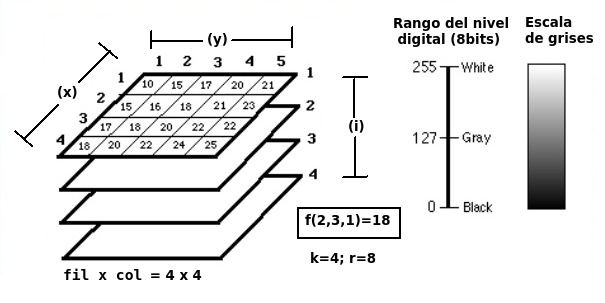
\includegraphics[width=0.7	\textwidth]{imagenes/cap3/imagen_satelital_k4.png}
				\label{fig:imagenMultiespectral}
			\end{figure}
			
		\end{frame}
		
		
		%%%%%%%%%%%%%
		\begin{frame}
			\frametitle{Im\'agenes satelitales\\Correcciones a las im\'agenes satelitales}		
			
			\begin{itemize}
				\item Correcci\'on geom\'etrica
				\begin{figure}[H]
					\centering
					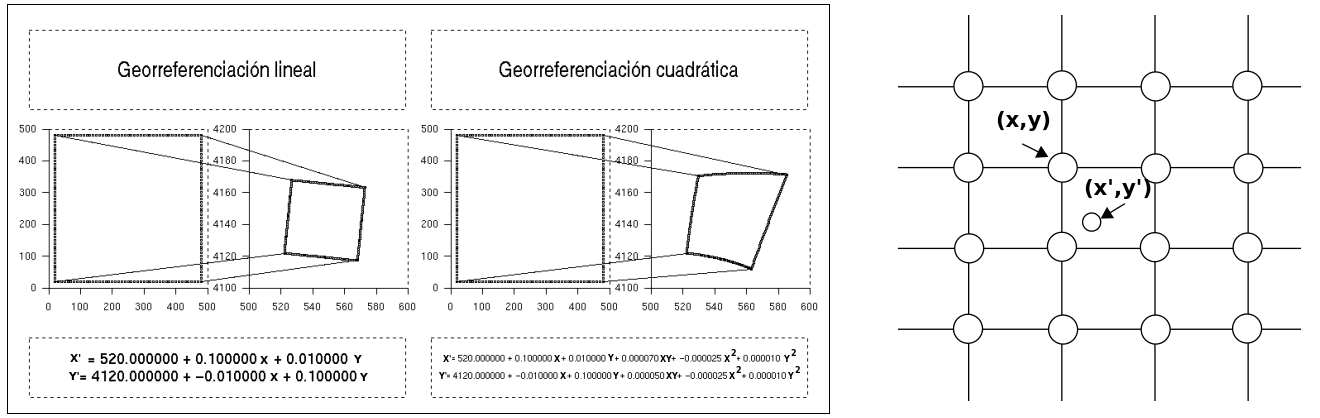
\includegraphics[width=0.7	\textwidth]{imagenes/cap3/correccImagenes.png}
					\label{fig:intPolEcua}
				\end{figure}
				\item Correcci\'on radiom\'etrica
				\begin{figure}[H]
					\centering
					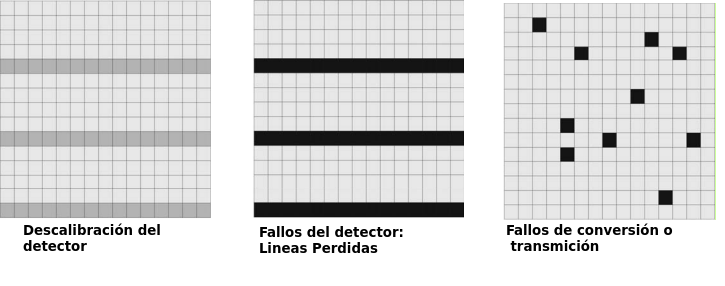
\includegraphics[width=0.5	\textwidth]{imagenes/cap3/correcError.png}
					\label{fig:vecinoMasCercano2}
				\end{figure}						
			\end{itemize}
		\end{frame}			
		
		%%%%%%%%%%%%%
		\begin{frame}
			\frametitle{Im\'agenes satelitales\\\'Indice de vegetaci\'on diferencial normalizada (NDVI)}		
			
			
			
			\onslide<1->{
				\begin{figure}[H]
					\centering
					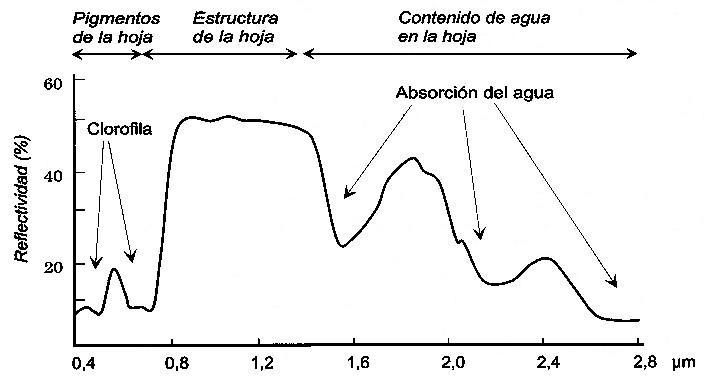
\includegraphics[width=0.6 \textwidth]{imagenes/cap3/Firma_espectral_vegetacion_vigorosa.jpg}
					\label{fig:firmaVegetacion}
				\end{figure}}
				
				\onslide<2->{
					Sea una funci\'on $ ndvi_{f}:(x,y) \longrightarrow [-1,1] $ que determina el NDVI de la imagen satelital $ f $ en cada coordenada espacial $ (x,y) $ definida por la siguiente expresi\'on:
					\begin{equation}
					\label{e:ndvi}
					ndvi_{f}(x,y)=\dfrac{f(x,y,IRc)-f(x,y,R)}{f(x,y,IRc)+f(x,y,R)}
					\end{equation}}					
				
			\end{frame}
			
			
			%%%%%%%%%%%%%
			\begin{frame}
				\frametitle{Im\'agenes satelitales\\Nomalizaci\'on Radiom\'etrica}		
				\onslide<1->{
					Una secuencia multitemporal esta definido por $ \{f_{t}\}_{t \in \mathbb{N}} $, que representa una secuencia de im\'agenes satelitales de la misma zona en diferentes tiempos.}
				\onslide<2->{
					\begin{figure}[H]
						\centering
						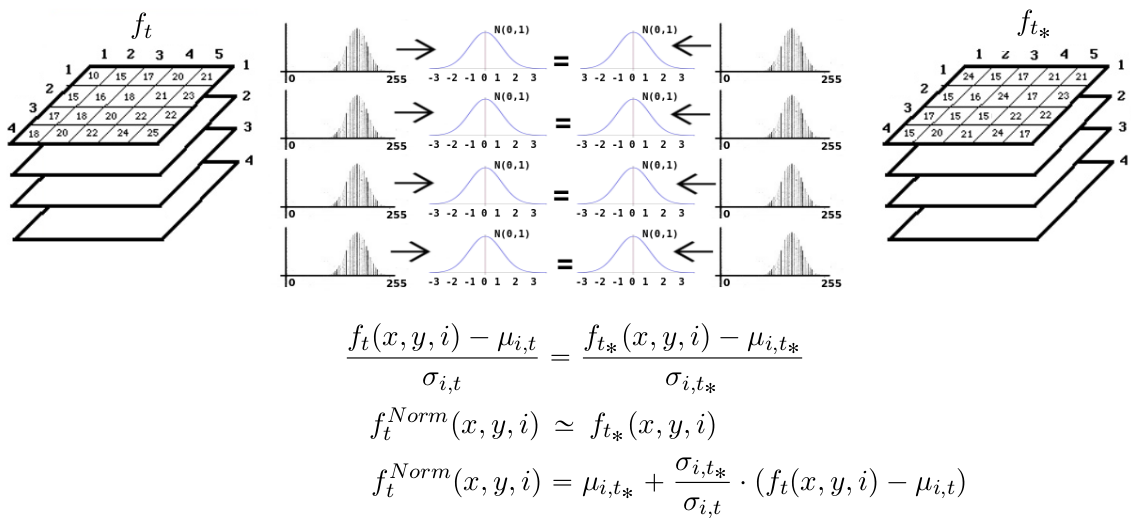
\includegraphics[width=1.0	\textwidth]{imagenes/cap4/normalizacionZecuacion_3.png}	
						\label{fig:normProceso}
					\end{figure}}
					
				\end{frame}				
				
				%%%%%%%%%%%%%
				\section{Metodolog\'ia propuesta}
				\begin{frame}
					\frametitle{Metodolog\'ia propuesta}						
					\begin{figure}[H]
						\centering
						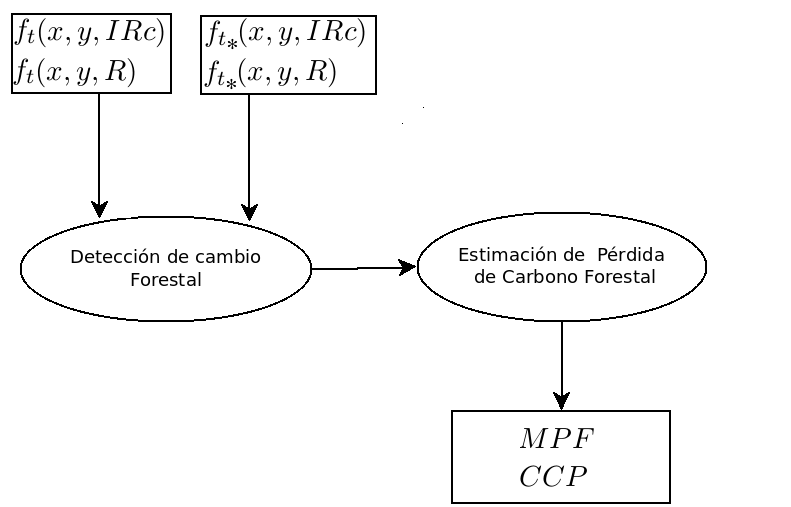
\includegraphics[width=0.8	\textwidth]{imagenes/cap4/metodologiaCarbono_3.png}
						\label{fig:metodologiapc}
					\end{figure}
				\end{frame}				
				
				%%%%%%%%%%%%%
				\begin{frame}
					\frametitle{Metodolog\'ia propuesta\\Detecci\'on de cambio Forestal }						
					\only<1>{
						\textbf{Detecci\'on de cambio}
						\begin{figure}[H]
							\centering
							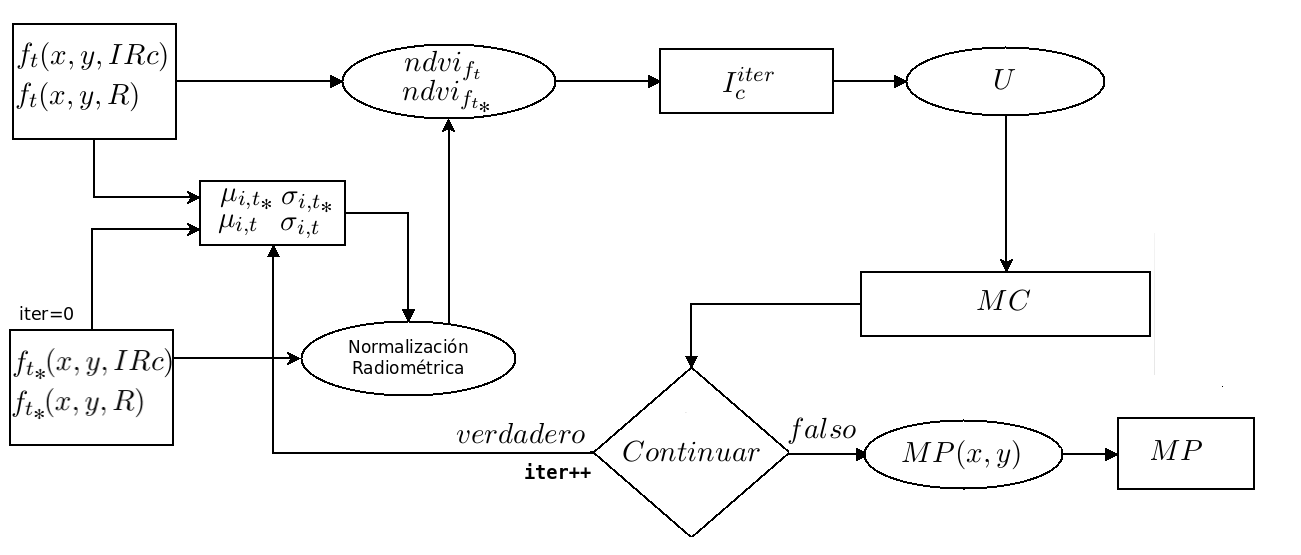
\includegraphics[width=1.0 \textwidth]{imagenes/cap4/deteccionCambio_4.png}
							\label{fig:deteccionCambio}
						\end{figure}}
						\only<2>{
							\textbf{Discriminaci\'on Forestal}
							\begin{figure}[H]
								\centering
								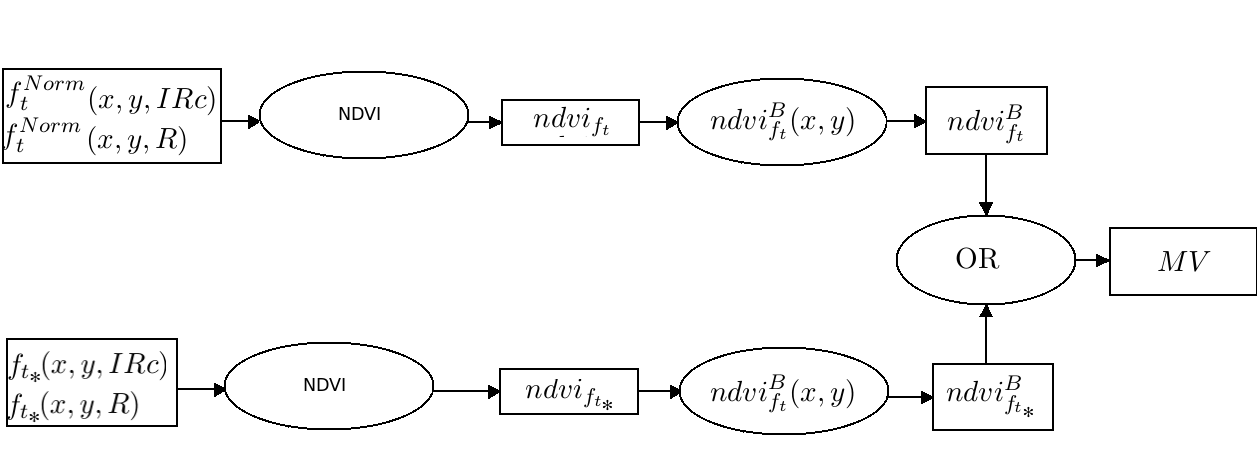
\includegraphics[width=1.0	\textwidth]{imagenes/cap4/discriminacionForestal_2.png}
								\label{fig:discrimForestal}
							\end{figure}}
							\only<3>{
								\textbf{Mascara de P\'erdida Forestal}
								\begin{figure}[H]
									\centering
									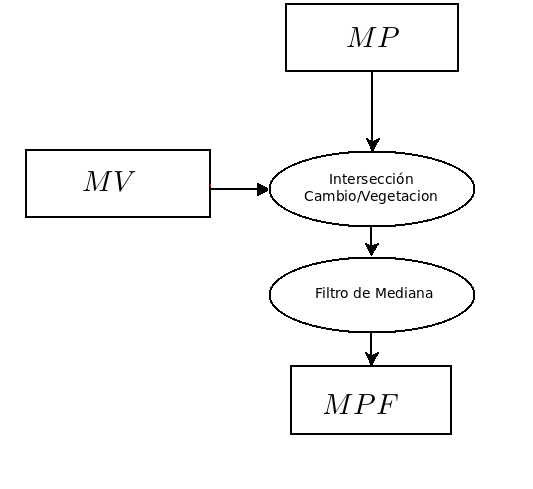
\includegraphics[width=0.6	\textwidth]{imagenes/cap4/interseccionPerdida.png}
									\label{fig:intersPerdida}
								\end{figure}}
							\end{frame}				
							
							%%%%%%%%%%%%%
							\begin{frame}
								\frametitle{Metodolog\'ia propuesta\\ Estimaci\'on de p\'erdida de carbono forestal}						
								Sea $ C:(x,y) \longrightarrow \{ [-\infty,\infty]\}$ la cantidad de carbono, en toneladas por hect\'area, para la coordenada $ (x,y) $, se tiene que: 
								\onslide<1->{
									\begin{equation}\label{ec:regreLinelCarb}
									C(x,y)=h+m \times ndvi_{f}(x,y)
									\end{equation}}
								\onslide<2->{
									\begin{equation}
									\label{e:restaCarm}
									C_{t}(x,y) - C_{t_{*}}(x,y)= m \times (ndvi_{f_{t}}(x,y) - ndvi_{f_{t_{*}}}(x,y))
									\end{equation}}
								\onslide<3->{
									\begin{equation}\label{ec:carbonom}
									PC(x,y) = m \times Ic(x,y)
									\end{equation}}
								\onslide<4->{
									\begin{equation}\label{ec:carbonoFinalm}
									PC(x,y) = 0.09 \times m \times Ic(x,y)
									\end{equation}}
								\onslide<5->{
									\begin{equation}\label{ec:carbonoFinalsumatoriam}
									CCP = \Sigma_{c=0}^{fil}\Sigma_{d=0}^{col} PC(x,y)
									\end{equation}}
							\end{frame}	
							
							%%%%%%%%%%%%%
							\begin{frame}
								\frametitle{Metodolog\'ia propuesta\\ Ejemplo}						
								\only<1>{
									\begin{figure}[H]
										\centering
										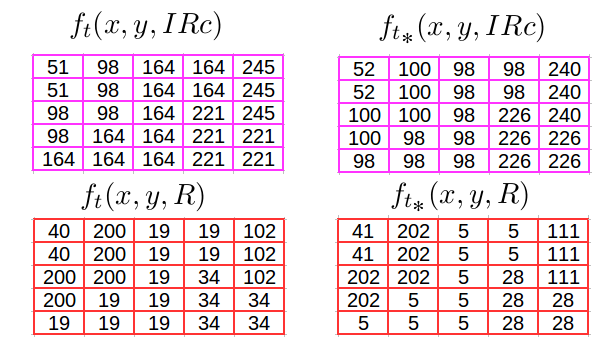
\includegraphics[width=0.6	\textwidth]{imagenes/cap4/ejemplo_entrada.png}
										\label{fig:ejemplo_1}
									\end{figure}}
									\only<2>{\begin{figure}[H]
											\centering
											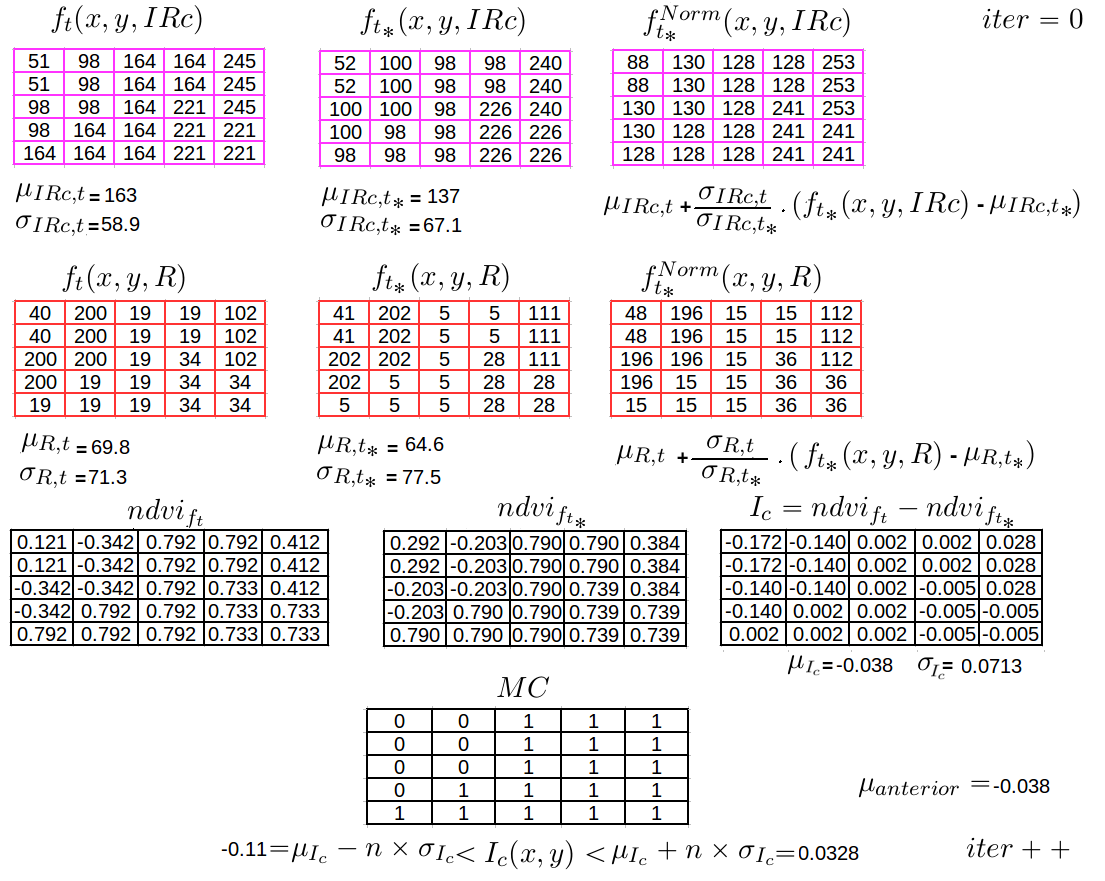
\includegraphics[width=0.75	\textwidth]{imagenes/cap4/ejemplo_iteracion_1.png}
											\label{fig:ejemplo_2}
										\end{figure}}					
										\only<3>{\begin{figure}[H]
												\centering
												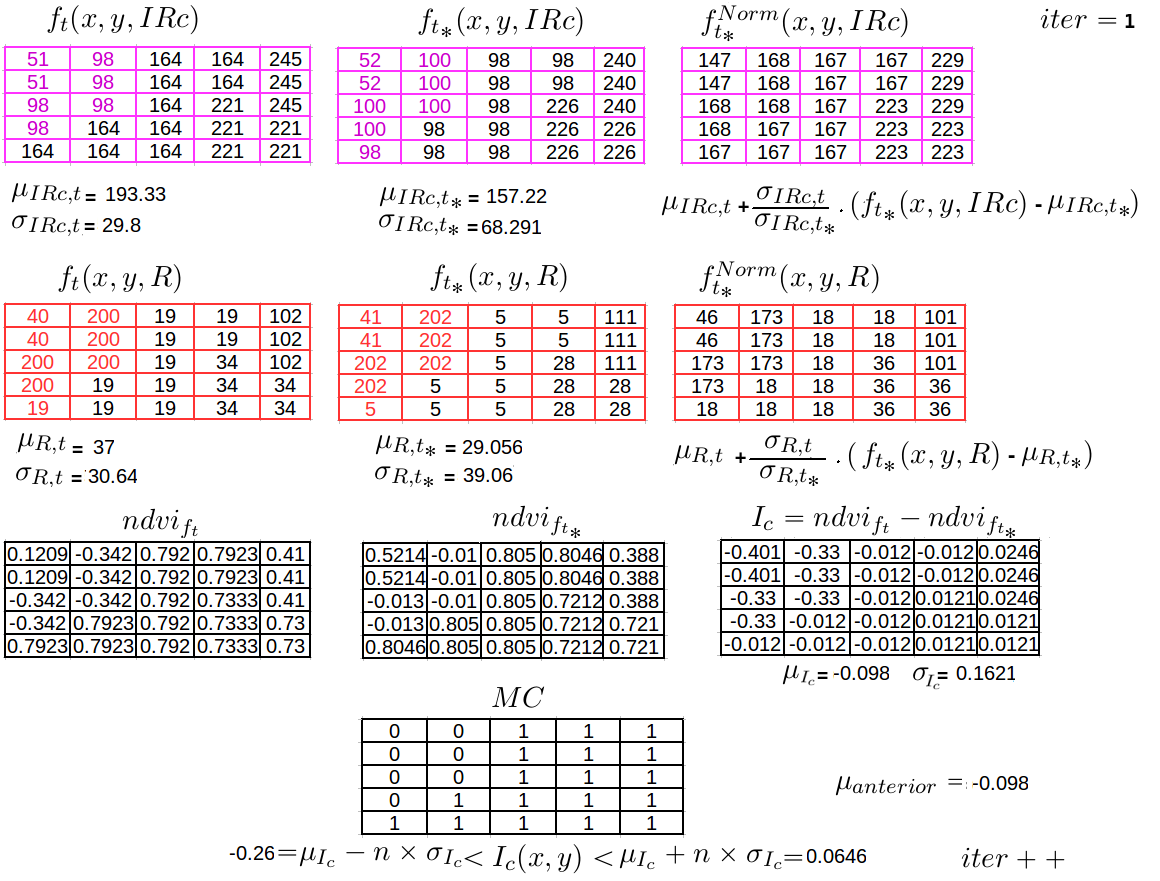
\includegraphics[width=0.8	\textwidth]{imagenes/cap4/ejemplo_iteracion_2.png}
												\label{fig:ejemplo_3}
											\end{figure}}
											\only<4>{\begin{figure}[H]
													\centering
													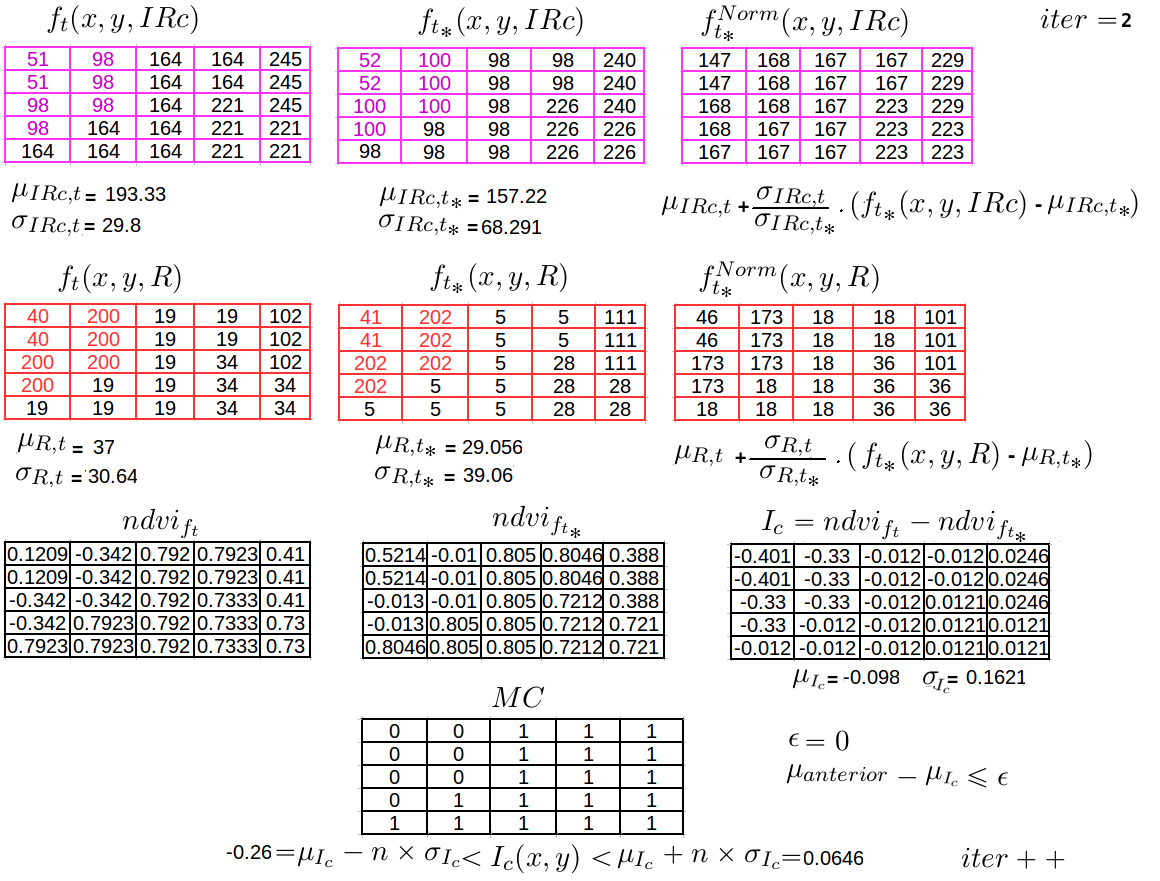
\includegraphics[width=0.8	\textwidth]{imagenes/cap4/ejemplo_iteracion_3.png}
													\label{fig:ejemplo_4}
												\end{figure}}
												\only<5>{\begin{figure}[H]
														\centering
														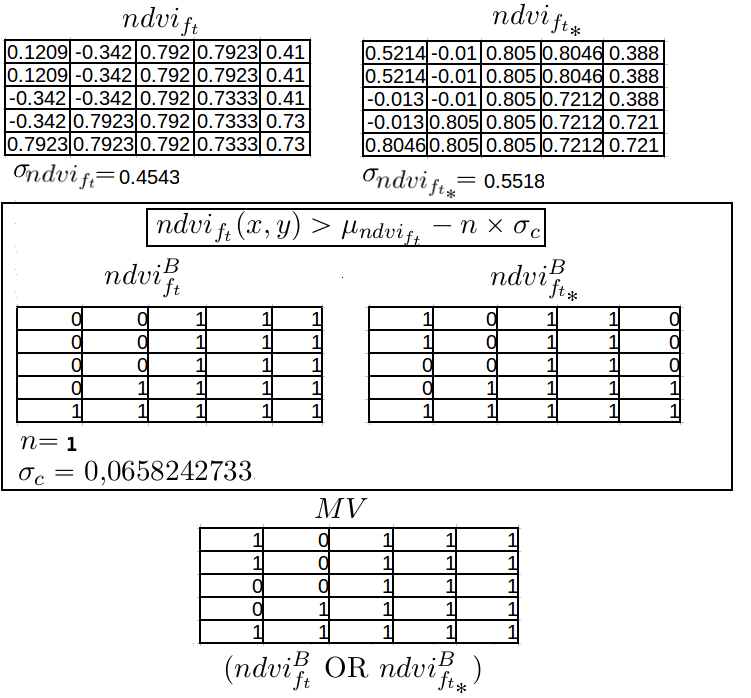
\includegraphics[width=0.6	\textwidth]{imagenes/cap4/ejemplo_ndvi.png}
														\label{fig:ejemplo_5}
													\end{figure}}
													\only<6>{\begin{figure}[H]
															\centering
															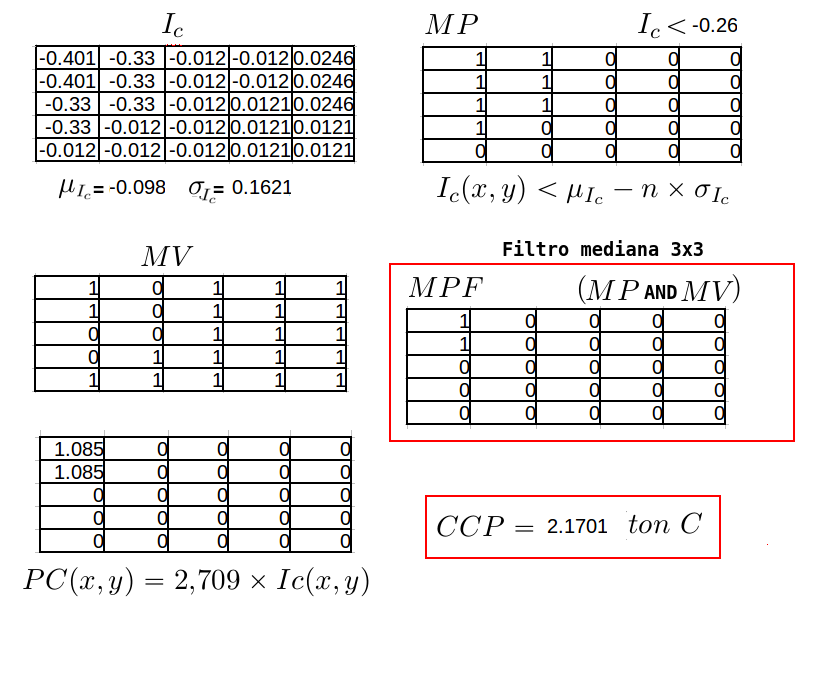
\includegraphics[width=0.8	\textwidth]{imagenes/cap4/ejemplo_resultado.png}
															\label{fig:ejemplo_6}
														\end{figure}}
														
													\end{frame}					
													
													%%%%%%%%%%%%%
													\section{M\'etricas de evaluaci\'on}
													\begin{frame}
														\frametitle{M\'etricas de evaluaci\'on}		
														\only<1>{
															\begin{table}[H]
																\centering
																\begin{tabular}{|
																		>{\columncolor[HTML]{EFEFEF}}l |p{2cm}|p{2cm}|p{2cm}|}
																	\hline
																	\textbf{Categorias}             & \cellcolor[HTML]{EFEFEF}\textbf{Perdida (VT)} & \cellcolor[HTML]{EFEFEF}\textbf{No Perdida (VT)} & \cellcolor[HTML]{EFEFEF}\textbf{Total (VT)} \\ \hline
																	\textbf{Perdida (Algoritmo)}    & TP                                            & FP                                               & P                                           \\ \hline
																	\textbf{No Perdida (Algoritmo)} & FN                                            & TN                                               & N                                           \\ \hline
																	\textbf{Total (Algoritmo)}      & P'                                            & N'                                               & Total                                       \\ \hline
																\end{tabular}
																\caption{Matriz de Confusi\'on}
																\label{t:matrizConfusion}
															\end{table}}
															
															\only<2>{
																\textbf{Porcentaje de precisi\'on global (GA)}
																\begin{equation}
																GA = \frac{TP+TN}{T+F}\cdot100
																\end{equation}}
															\only<3>{
																\textbf{Coeficiente Kappa}
																\begin{equation}
																KAPPA=\dfrac{Total \times (TP+TN)-(P \times P'+N \times N')}{Total^{2} \times (P \times P'+N \times N')}
																\end{equation}
																\begin{table}[H]
																	\centering
																	\begin{tabular}{|l|l|}
																		\hline
																		\rowcolor[HTML]{EFEFEF} 
																		\textbf{Coeficiente Kappa} & \textbf{Fuerza de la concordancia} \\ \hline
																		0,00                       & Pobre                              \\ \hline
																		0,01-0,20                  & Leve                               \\ \hline
																		0,21-0,40                  & Aceptable                          \\ \hline
																		0,41-0,60                  & Moderada                           \\ \hline
																		0,61-80                    & Considerable                       \\ \hline
																		0,81-1,00                  & Casi perfecta                      \\ \hline
																	\end{tabular}
																	\caption{Valoraci\'on del coeficiente kappa.}
																	\label{t:kappaTable}
																\end{table}
															}
															
														\end{frame}								
														
														%%%%%%%%%%%%%
														\section{Pruebas y resultados experimentales}
														\begin{frame}
															\frametitle{Pruebas y resultados experimentales\\Umbral de Vegetaci\'on}						
															\only<1>{
																\begin{figure}[H]
																	\centering
																	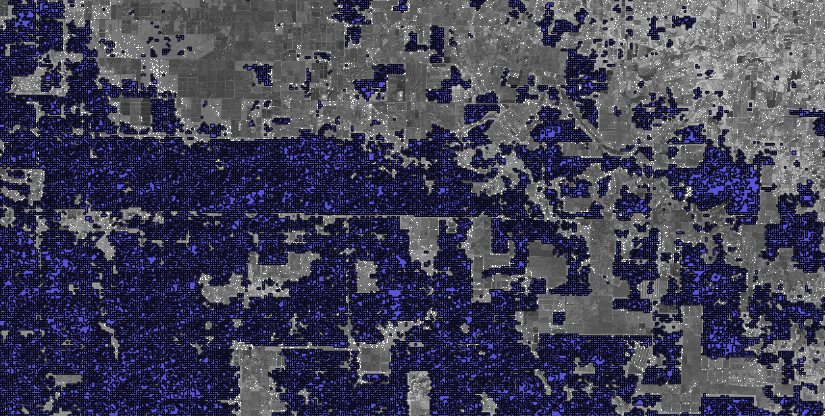
\includegraphics[width=0.8	\textwidth]{imagenes/cap5/mascaraVCF.png}
																	\label{fig:mascVCf}
																\end{figure}
															}
															\only<2>{
																\begin{figure}[H]
																	\centering
																	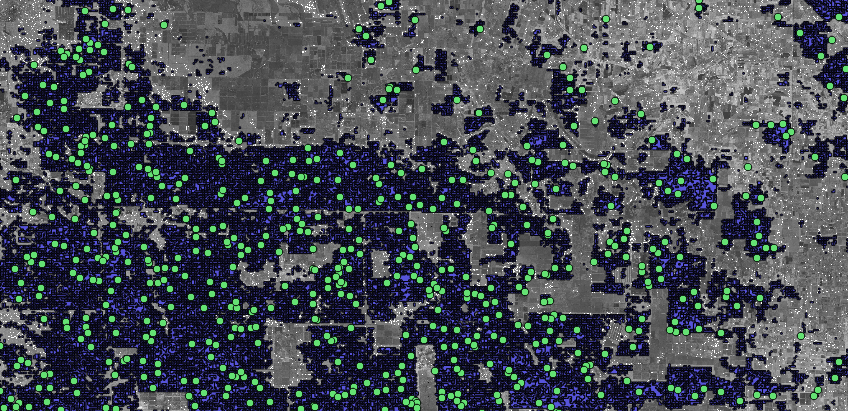
\includegraphics[width=0.8	\textwidth]{imagenes/cap5/vcfAleatorio.png}
																	\label{fig:aleatorioVCf}
																\end{figure}
															}
															\only<3>{
																\begin{table}[H]
																	\scalebox{0.6}{
																		\centering
																		\begin{tabular}{|l|l|l|}
																			\hline
																			\rowcolor[HTML]{EFEFEF} 
																			\multicolumn{3}{|c|}{\cellcolor[HTML]{EFEFEF}\textbf{A\~{n}o 1986}}        \\ \hline
																			\rowcolor[HTML]{EFEFEF} 
																			\textbf{VCF (\%)} & \textbf{$ \mu_{ndvi_{ft}} $} & \textbf{$ \sigma_{ndvi_{ft}} $} \\ \hline
																			50                & 0.356701              & 0.047891                   \\ \hline
																			40                & 0.344022              & 0.0507296                  \\ \hline
																			30                & 0.337696              & 0.061581                   \\ \hline
																			20                & 0.339586              & 0.0632055                  \\ \hline
																			10                & 0.335528              & 0.0727573                  \\ \hline
																			\rowcolor[HTML]{EFEFEF} 
																			\multicolumn{3}{|c|}{\cellcolor[HTML]{EFEFEF}\textbf{A\~{n}o 1990}}        \\ \hline
																			\rowcolor[HTML]{EFEFEF} 
																			\textbf{VCF (\%)} & \textbf{$ \mu_{ndvi_{ft}} $} & \textbf{$ \sigma_{ndvi_{ft}} $} \\ \hline
																			50                & 0.278804              & 0.0631834                  \\ \hline
																			40                & 0.264651              & 0.0679451                  \\ \hline
																			30                & 0.254145              & 0.0742348                  \\ \hline
																			20                & 0.252186              & 0.0759032                  \\ \hline
																			10                & 0.251421              & 0.0796667                  \\ \hline
																			\rowcolor[HTML]{EFEFEF} 
																			\multicolumn{3}{|c|}{\cellcolor[HTML]{EFEFEF}\textbf{A\~{n}o 1990}}        \\ \hline
																			\rowcolor[HTML]{EFEFEF} 
																			\textbf{VCF (\%)} & \textbf{$ \mu_{ndvi_{ft}} $} & \textbf{$ \sigma_{ndvi_{ft}} $} \\ \hline
																			50                & 0.0202133             & 0.0572825                  \\ \hline
																			40                & 0.0104289             & 0.0608757                  \\ \hline
																			30                & -0.00337075           & 0.066776                   \\ \hline
																			20                & -0.00663188           & 0.0695777                  \\ \hline
																			10                & -0.0103891            & 0.0757546                  \\ \hline
																		\end{tabular}}
																		\label{t:vcfNdvi}
																	\end{table}
																	$ \sigma_{c} = 0.0658242733 $
																}
															\end{frame}		
															
															\begin{frame}
																\frametitle{Pruebas y resultados experimentales\\Estimaci\'on de p\'erdida de carbono forestal}						
																\only<1>{
																	\begin{figure}[H]
																		\centering
																		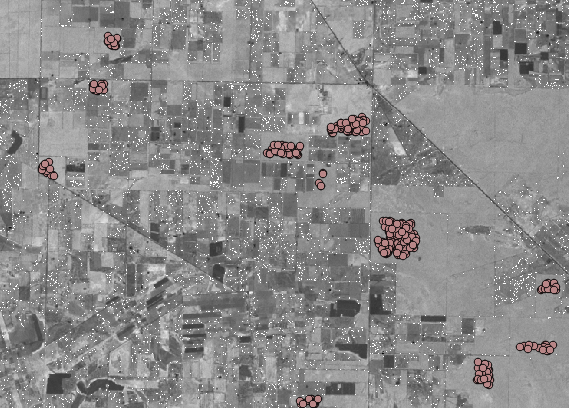
\includegraphics[width=0.8	\textwidth]{imagenes/cap5/carbNdvi.png}
																		\label{fig:aleatorioCrb}
																	\end{figure}
																}
																\only<2>{
																	\begin{figure}[H]
																		\centering
																		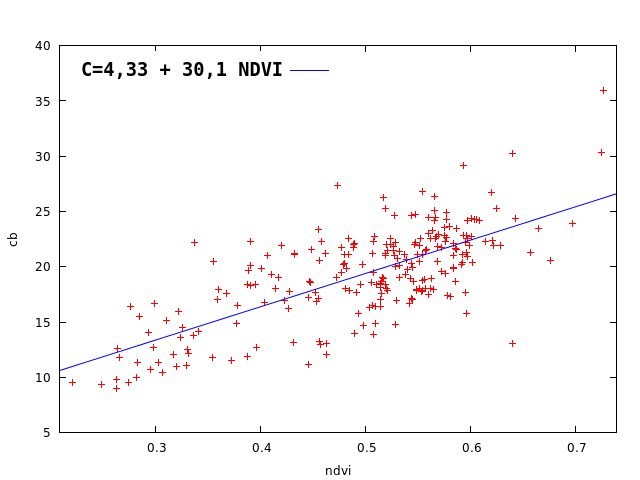
\includegraphics[width=0.8	\textwidth]{imagenes/cap4/ndviCarb.png}
																		\caption{Regresi\'on Lineal. $ X=NDVI, Y=TonC/ha $}
																		\label{fig:linealCar}
																	\end{figure}
																	$ r^{2}=0.509125 $
																}
																\only<3>{
																	\begin{equation}\label{ec:regreLinelCarbExp}
																	C(x,y)=4.33+30.1 \times ndvi_{f}(x,y)
																	\end{equation}
																	\begin{equation}\label{ec:carbonoFinalmExp}
																	PC(x,y) = 2.709 \times Ic(x,y)
																	\end{equation}
																}
																
															\end{frame}		
															
															\begin{frame}
																\frametitle{Pruebas y resultados experimentales\\Prueba experimental}						
																\only<1>{
																	\begin{figure}[H]
																		\centering
																		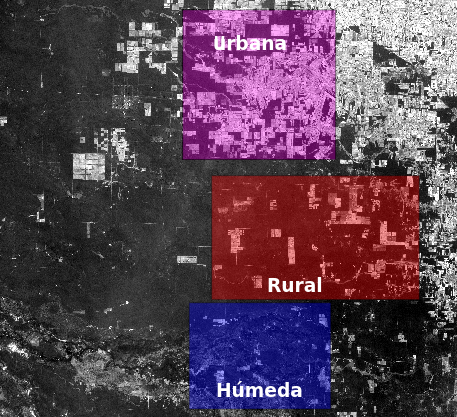
\includegraphics[width=0.55	\textwidth]{imagenes/cap5/zonas.png}
																		\caption{\'Areas de los sectores empleados para los experimentos.}
																		\label{fig:zonasEva}
																	\end{figure}
																}
																\only<2>{
																	\begin{table}[H]
																		\centering
																		
																		\begin{tabular}{|l|l|l|}
																			\hline
																			\rowcolor[HTML]{EFEFEF} 
																			\textbf{Sat\'elite} & \textbf{Path-row} & \textbf{Fecha}  \\ \hline
																			Landsat-5         & 228-76            & 1-26-199       \\ \hline
																			Landsat-7         & 229-76            & 8-17-1999      \\ \hline
																		\end{tabular}
																		\label{t:pathRow}
																	\end{table}
																}
																\only<3>{
																	\begin{figure}[H]
																		\centering
																		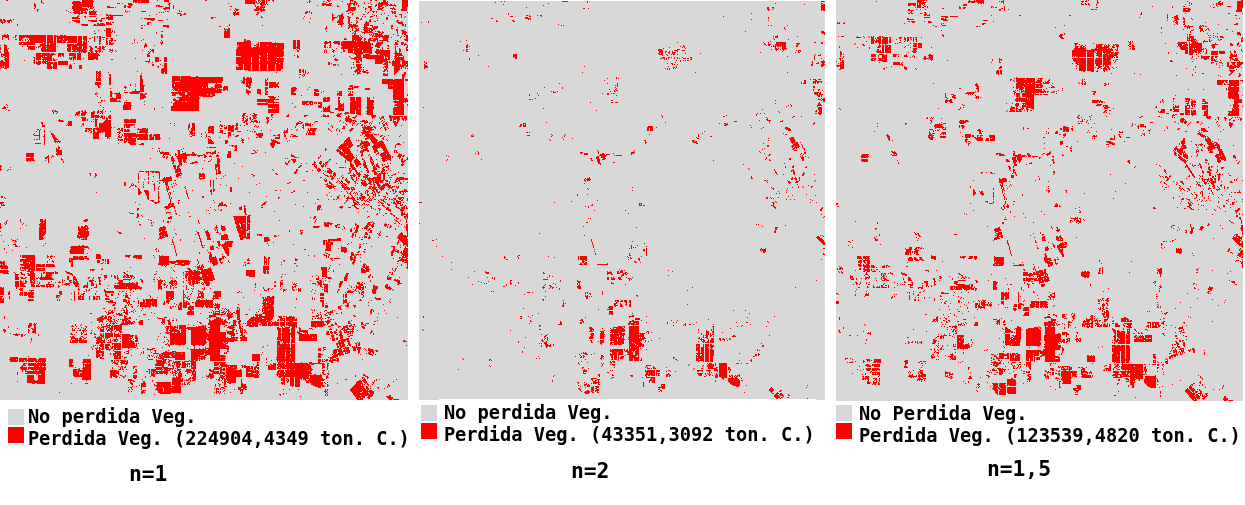
\includegraphics[width=1.0	\textwidth]{imagenes/cap5/res_zona_urbana.png}
																		\caption{\'Area Urbana. Mapa de p\'erdida forestal y toneladas de carbono perdidos.}
																		\label{fig:ubana}
																	\end{figure}
																}
																\only<4>{
																	\begin{figure}[H]
																		\centering
																		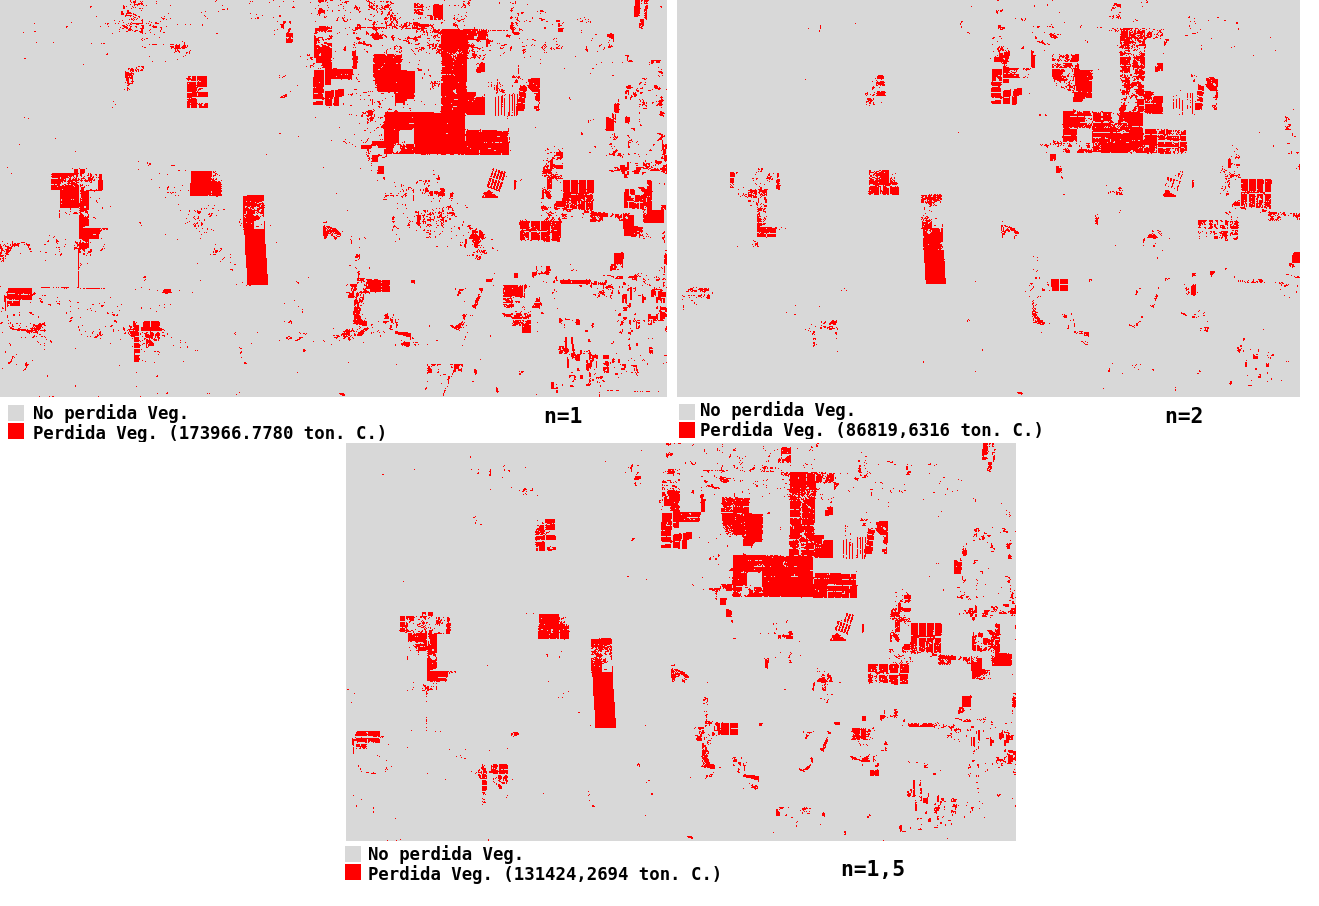
\includegraphics[width=0.7	\textwidth]{imagenes/cap5/res_zona_rural.png}
																		\caption{\'Area Rural. Mapa de p\'erdida forestal y toneladas de carbono perdidos}
																		\label{fig:rural}
																	\end{figure}
																}
																\only<5>{
																	\begin{figure}[H]
																		\centering
																		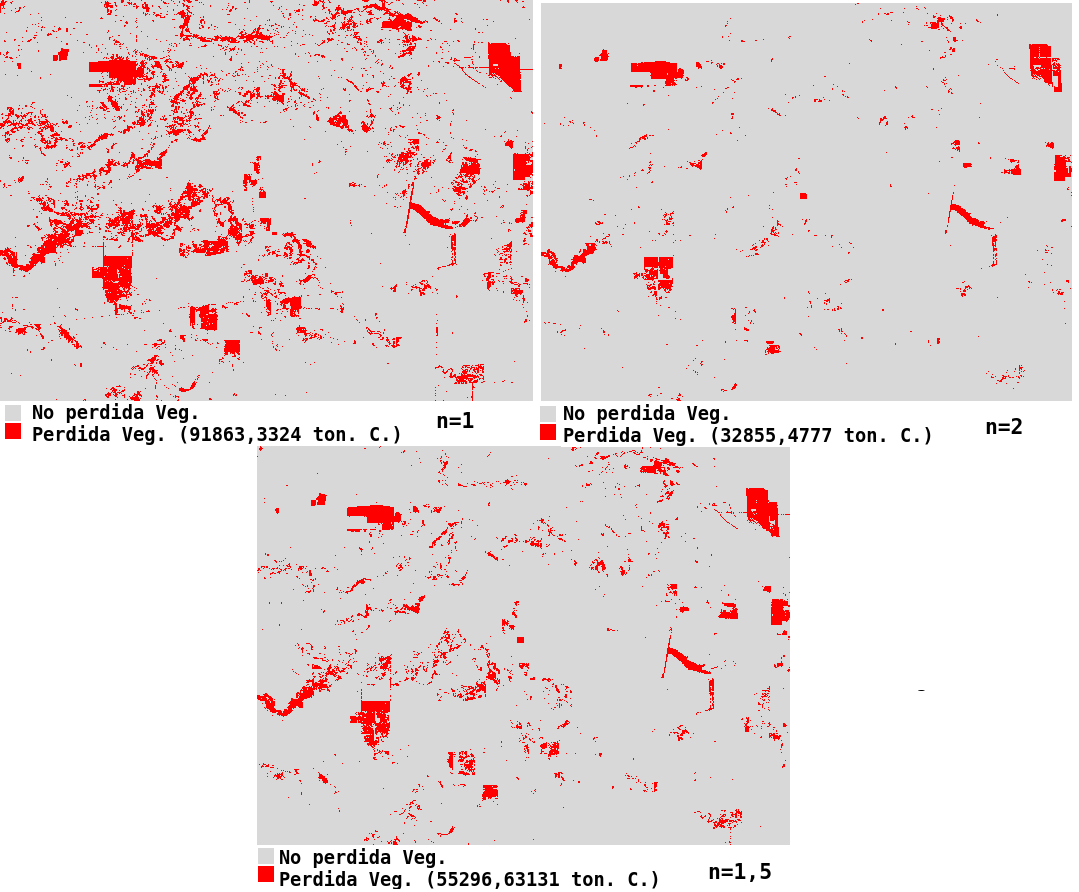
\includegraphics[width=0.6	\textwidth]{imagenes/cap5/res_zona_humeda.png}
																		\caption{\'Area H\'umeda. Mapa de p\'erdida forestal y toneladas de carbono perdidos}
																		\label{fig:humeda}
																	\end{figure}
																	
																}
																\only<6>{
																	\begin{figure}[H]
																		\centering
																		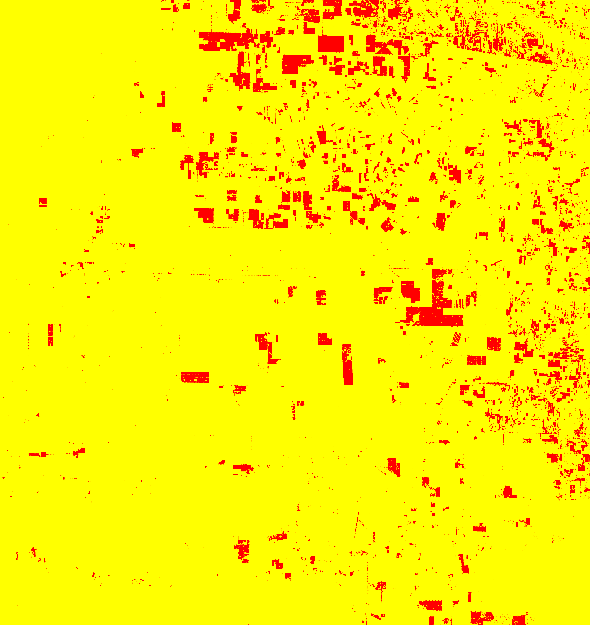
\includegraphics[width=0.5	\textwidth]{imagenes/cap5/pcfp.png}
																		\caption{Re-clasificaci\'on de la imagen PFCP. Perdida = 1, Otros=0}
																		\label{fig:pfcp}
																	\end{figure}
																}
																\only<7>{
																	\begin{table}[H]
																		\scalebox{0.7}{
																			\centering
																			
																			\begin{tabular}{|l|l|l|}
																				\hline
																				\rowcolor[HTML]{EFEFEF} 
																				\multicolumn{3}{|l|}{\cellcolor[HTML]{EFEFEF}\textbf{N=1}}   \\ \hline
																				\rowcolor[HTML]{EFEFEF} 
																				\textbf{\'Area}  & \textbf{Kappa}  & \textbf{Precisi\'on Global} \\ \hline
																				Urbano         & 0.476389        & 84.257452                 \\ \hline
																				Rural          & 0.65782         & 93.82121                  \\ \hline
																				H\'umeda         & 0.301541        & 90.624794                 \\ \hline
																				\rowcolor[HTML]{EFEFEF} 
																				\multicolumn{3}{|l|}{\cellcolor[HTML]{EFEFEF}\textbf{N=1.5}} \\ \hline
																				\rowcolor[HTML]{EFEFEF} 
																				\textbf{\'Area}  & \textbf{Kappa}  & \textbf{Precisi\'on Global} \\ \hline
																				Urbano         & 0.315273        & 83.514875                 \\ \hline
																				Rural          & 0.671753        & 94.899171                 \\ \hline
																				H\'umeda         & 0.425555        & 96.693648                 \\ \hline
																				\rowcolor[HTML]{EFEFEF} 
																				\multicolumn{3}{|l|}{\cellcolor[HTML]{EFEFEF}\textbf{N=2}}   \\ \hline
																				\rowcolor[HTML]{EFEFEF} 
																				\textbf{\'Area}  & \textbf{Kappa}  & \textbf{Precisi\'on Global} \\ \hline
																				Urbano         & 0.09368         & 81.642457                 \\ \hline
																				Rural          & 0.570687        & 94.33648                  \\ \hline
																				H\'umeda         & 0.425555        & 96.693648                 \\ \hline
																			\end{tabular}}
																			\caption{Coeficiente Kappa y precisi\'on Global obtenidos.}
																			\label{t:kappaGa}
																		\end{table}
																	}
																	\only<8>{
																		\begin{figure}[H]
																			\centering
																			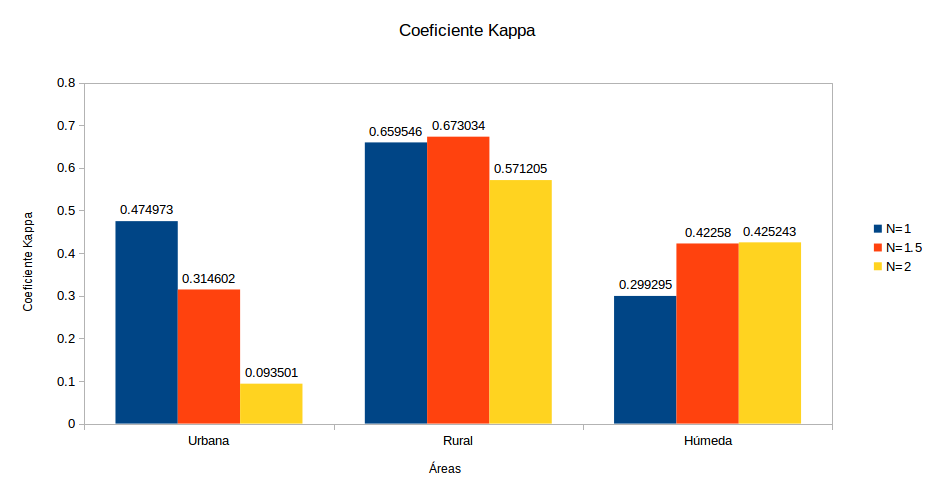
\includegraphics[width=0.9	\textwidth]{imagenes/cap5/kappaGrafico.png}
																			\caption{Coeficiente Kappa por cada \'Area y tolerancia.}
																			\label{fig:kappaGrafico}
																		\end{figure}
																	}
																	\only<9>{
																		\begin{figure}[H]
																			\centering
																			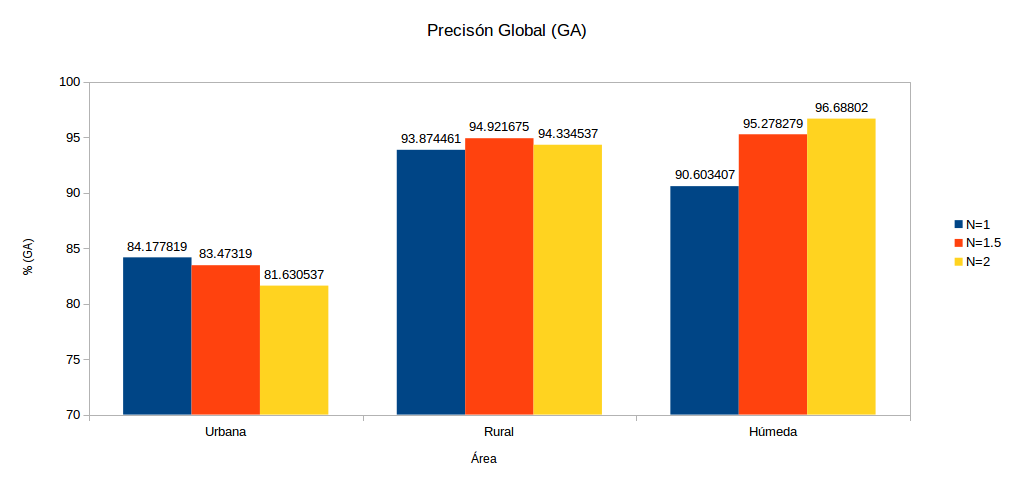
\includegraphics[width=0.9	\textwidth]{imagenes/cap5/gaGrafico.png}
																			\caption{GA por cada \'Area y tolerancia.}
																			\label{fig:gaGrafico}
																		\end{figure}
																	}
																	
																\end{frame}										
																\section{Conclusiones y trabajos futuros}	
																\begin{frame}
																	\frametitle{Conclusiones y trabajos futuros\\Conclusiones}						
																	
																	\begin{itemize} \scriptsize
																		\item La normalizaci\'on radiom\'etrica permite que los pixeles de una secuencia multitemporal sean semejantes. Los indices de cambios obtenidos de la comparaci\'on multitemporal posibilitan obtener variables cualitativas a partir de umbrales elaborados por par\'ametros estad\'isticos extra\'idos de la misma imagen de cambio $ I_{c} $. La iteraci\'on permite automatizar la detecci\'on de cambio, ya que el proceso normaliza repetidamente las im\'agenes teniendo en cuenta solo los pixeles que no sufrieron cambio en el tiempo, optimizando y mejorando la comparaci\'on multitemporal.
																		\item El an\'alisis estad\'istico realizado a las im\'agenes satelitales VCF y Landsat posibilitaron determinar a la desviaci\'on est\'andar de los NDVI calculados, como una constante que permite transforman las variables cuantitativas (NDVI) a variables cualitativas (vegetaci\'on/no vegetaci\'on).
																		\item El an\'alisis de regresi\'on permiti\'o encontrar una relaci\'on entre un \'indice de vegetaci\'on (NDVI) y el carbono (Mapa global de carbono), por lo que convertir el indice generado por las im\'agenes satelitales se resume en una ecuaci\'on que no implic\'o muestreo en campo ni estudios adicionales.
																		\item La detecci\'on de cambio forestal fue realizado mediante a la normalizaci\'on radiom\'etrica y comparaci\'on multitemporal de forma iterativa, donde el cambio forestal fue discriminado mediante el hallazgo de la desviaci\'on est\'andar de los NDVI. 
																		\item En la detecci\'on de cambio forestal los resultados obtenidos fueron comparados con la imagen PFCP, de manera a evaluar el proceso con m\'etricas de precisi\'on global y coeficiente kappa.
																	\end{itemize}

																	
																	
																\end{frame}															
																\begin{frame}
																	\frametitle{Conclusiones y trabajos futuros\\Trabajos futuros}						
																	
																	
																		\begin{itemize}
																			\item Se pretende que la metodolog\'ia propuesta siga mejorando en t\'erminos de pre-procesamiento de las im\'agenes satelitales, ante factores que influyan en el momento de captura de los datos hechas por sensores remotos como tambi\'en en t\'ecnicas que permita mejora la detecci\'on de cambio forestal.
																			\item Proponer t\'ecnicas que permitan detectar y eliminar nubosidad en las imagen satelitales.
																			\item Mejorar la precisi\'on global y el coeficiente kappa para zonas urbanas.
																			\item Dise\~{n}ar mejores t\'ecnicas que clasifique cobertura vegetal mediante la extracci\'on de indices en todas las bandas.
																			\item Adaptar la metodolog\'ia, de manera a que permita recibir im\'agenes satelitales con diferentes resoluciones radiom\'etricas.
																		\end{itemize}
																		
																	
																	
																	
																\end{frame}	
																
																
															\end{document} 